\section{QRS Complex detection}
Cardiologists use ECG signals to determine different arrhythmia conditions by visually examining the signal patterns. Therefore if we can detect those patterns using a computer program that can be used to predict different heart related problems. Such a program can operate on real time to monitor heart patients.  
 
One of the most basic pattern to detect is the QRS complex. Since QRS complex shows a high voltage change during a short time this is a very easy pattern to detect. However this is not straight forward since ECG signals can be effected from noise. There are some signal processing techniques \cite{pan1985real} developed to detect the QRS complex.  Most of these techniques typically consists of band pass filtering, differentiation, squaring and peak detection.

Mimic II data set \footnote{http://physionet.org/mimic2/} which is stored at physionet.org provides set of ECG signal records of ICU patients. These record sets can be downloaded from  physionet.org \footnote{http://www.physionet.org/faq.shtml} . Each record contains set of ECG signal records. These records can be accessed using WFDB package \footnote{http://physionet.org/physiotools/wfdb.shtml}. 

Next sections of this document shows how to process ECG signal data obtained for record 3000762 during the interval of 1000s to 1010s. This can be obtain using following command.

rdsamp -r 3000762/ -p -s 'II' -f 1000 -t 1010 -c 

This waveform can be represented looks like in Figure \ref{ecg_original} with time.

\begin{figure}
        \centering
        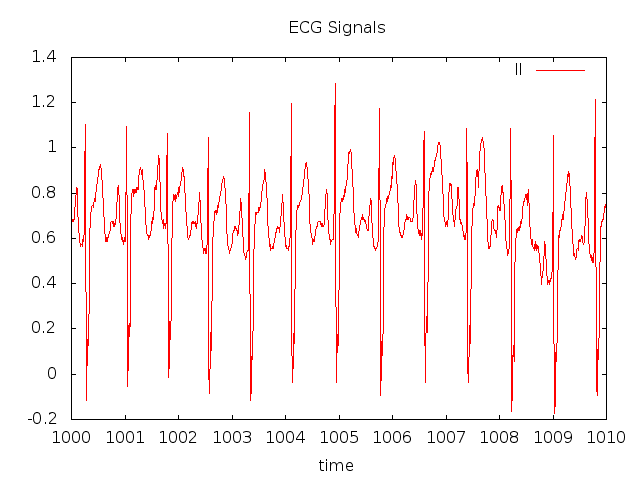
\includegraphics[width=\textwidth]{ecg_original.png}
        \caption{Original ECG}
        \label{ecg_original}
\end{figure}
\subsection{Band pass filtering}
As shown in Figure \ref{ecg_original} a typical ECG signal can have noise as well as some dc component. We can remove these by sending this signal through a band pass filter. It has been observed that ECG signals should have all its frequency components within the range of 5-15 Hz. Since sample frequency for the Mimic II data set waveforms is 200 Hz with need to design a band pass filter for 5-15 Hz for 200 Hz sample rate. Design a band pass filter from the scratch is complicated. However there is a python library which can be used to calculate the co efficients for a band pass filter as used here \footnote{http://www.cs.colostate.edu/eeg/data/json/doc/tutorial/build/html/downloads/bandpass.txt}. And can use the algorithm used here \footnote{http://code.google.com/p/stevens-ssp-plugin/wiki/DataStructure} to implement the band pass filter. 
Figure \ref{band_pass_filter} shows the signal after band pass filtering.
\begin{figure}
        \centering
        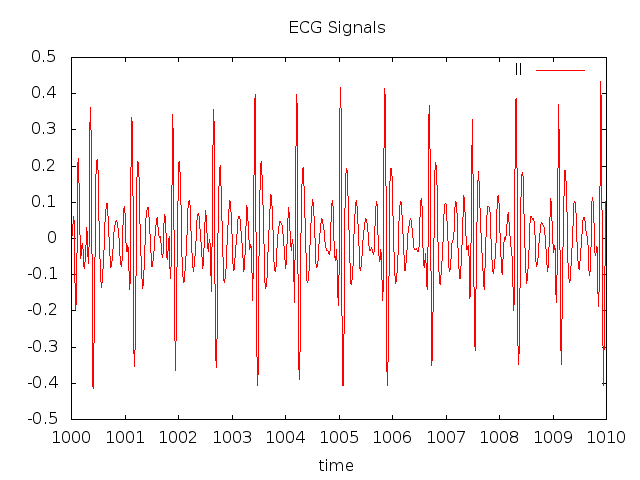
\includegraphics[width=\textwidth]{ecg_filtered.png}
        \caption{Band pass filtering}
        \label{band_pass_filter}
\end{figure}
\subsection{Differentiation}
After band pass filtering the signal can be differentiated to attenuate the higher variations. Figure \ref{differentiated_signal} shows the differentiated signal.
\begin{figure}
        \centering
        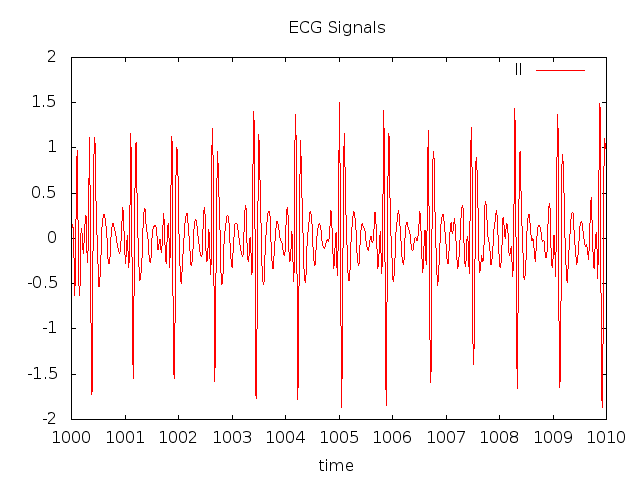
\includegraphics[width=\textwidth]{ecg_differentiated.png}
        \caption{Differentiated Signal}
        \label{differentiated_signal}
\end{figure}
\subsection{Squaring} 
Differentiated signal can be squared to remove the negative components. Figure \ref{squared_signal} shows the squared signal.
\begin{figure}
        \centering
        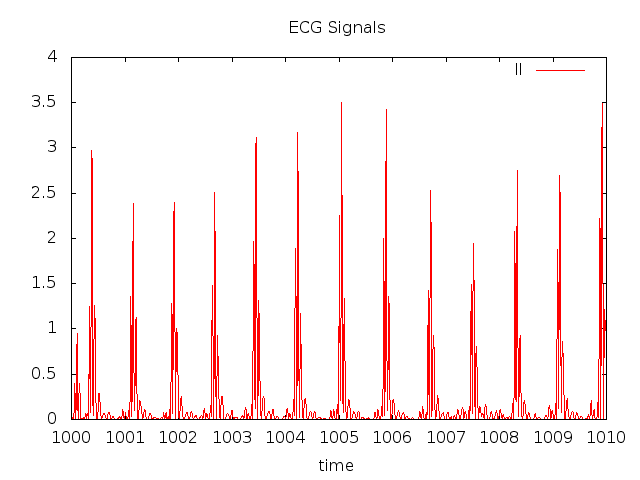
\includegraphics[width=\textwidth]{ecg_squared.png}
        \caption{Squared Signal}
        \label{squared_signal}
\end{figure}
\subsection{Integration}
Integration is a technique used to identify the peaks of the squared wave. In here integration window should be kept in a same distance as in QRS complex in order not to overlap with T wave. Figure \ref{integration_signal} shows the integrated signal.

After obtaining integrated signal peak points can be detected to find the QRS locations and hence the distance between two QRS complexes. Same type of peak detection can be done to find the distance of QRS complexes using band pass filters. The amplitute of band pass wave can be used to determine the amplitute of the signal. 
\begin{figure}
        \centering
        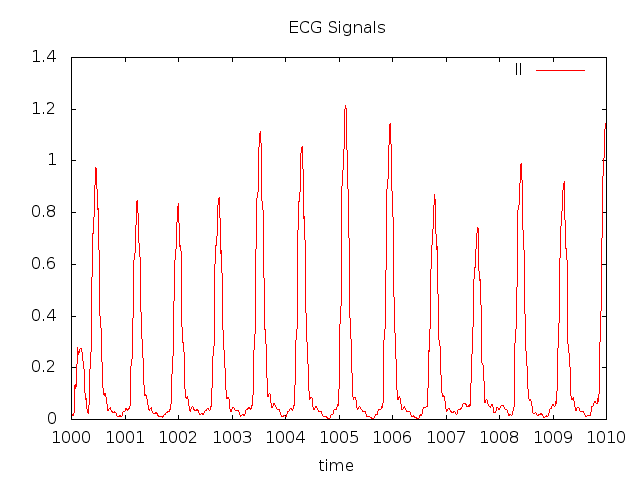
\includegraphics[width=\textwidth]{ecg_integration.png}
        \caption{Integration signal}
        \label{integration_signal}
\end{figure}
\subsection{Issues}
Although above technique works for the given data range, it does not work for all cases specially if there is noise or signal is not present for some time. Figure \ref{ecg1_original} and Figure \ref{ecg2_original} shows two of such cases and corresponding integration signals in Figure \ref{ecg1_integration} and Figure \ref{ecg2_integration}.

\begin{figure}
        \centering
        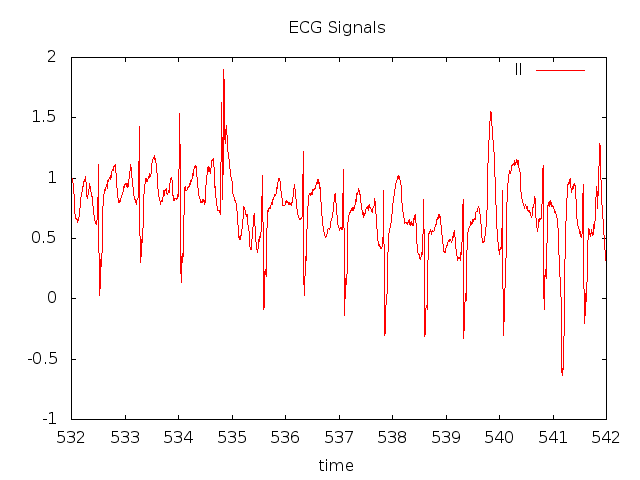
\includegraphics[width=\textwidth]{ecg1_original.png}
        \caption{Original signal}
        \label{ecg1_original}
\end{figure}
\begin{figure}
        \centering
        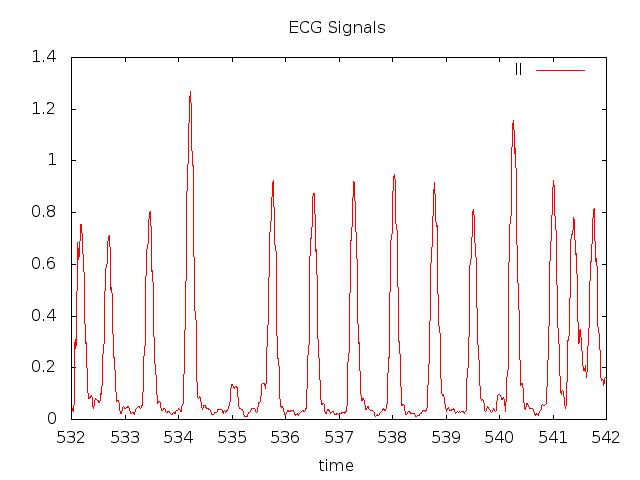
\includegraphics[width=\textwidth]{ecg1_integration.png}
        \caption{Integration signal}
        \label{ecg1_integration}
\end{figure}
\begin{figure}
        \centering
        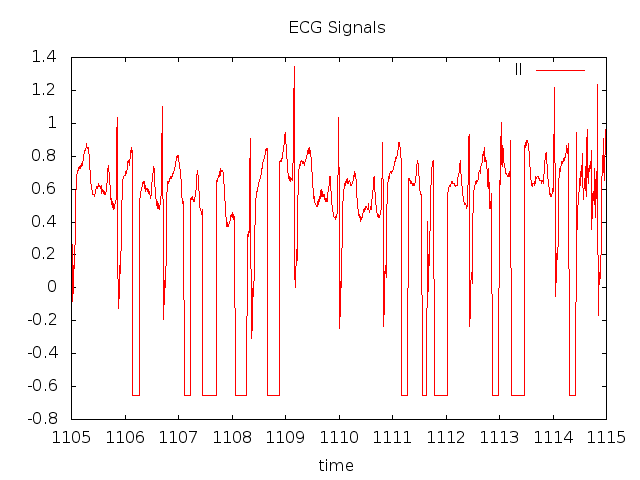
\includegraphics[width=\textwidth]{ecg2_original.png}
        \caption{Original signal}
        \label{ecg2_original}
\end{figure}
\begin{figure}
        \centering
        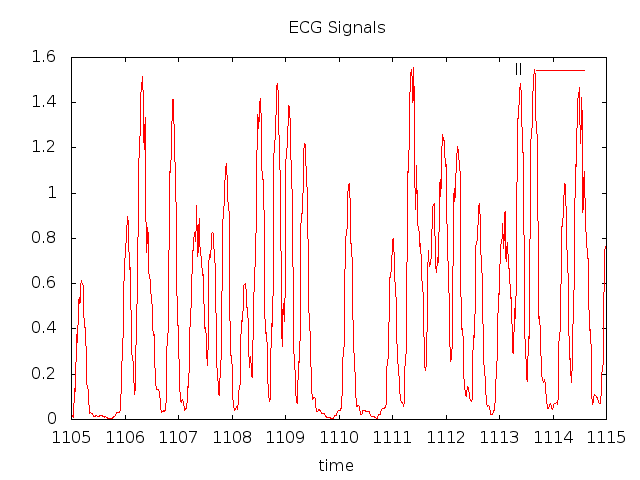
\includegraphics[width=\textwidth]{ecg2_integration.png}
        \caption{Integration signal}
        \label{ecg2_integration}
\end{figure}
